\section{Abstatung}\label{3}
Wird ein Vorgang zu (in der Regel) äquidistanten Zeitpunkten gemessen, so bezeichnet sich dies als Abtastung. Dies ist ein fundamentaler und in der Regel der erste Schritt für die Verarbeitung eines Signals. Im Folgenden werden zunächst die Grundlagen und die Theorie der Abtastung erörtert. Anschließend werden die wichtigsten Eigenschaften aufgezählt und bewiesen. In Abschnitt \ref{3.3} wird auf die Bedeutung dieser Eigenschaften im Kontext eines DSPs eingegangen. Zuletzt wird die Realisierung der Abtastung am Beispiel eines DSPs beschrieben, wobei Fokus auf die Problematiken und Lösungen gelegt wird.
\subsection{Theorie}\label{3.1}
Für jegliche Verarbeitung mithilfe eines DSPs, zur Übertragung mittels beispielsweise des 'Digital Audio Broadcastings' oder zur Minimierung des Speicherverbrauchs ist die Digitalisierung ein notwendiger Schritt in der Signalverarbeitung. 

\subsubsection{Analoge/Digitale Definitions- und Wertebereiche}
\begin{figure}
\centering
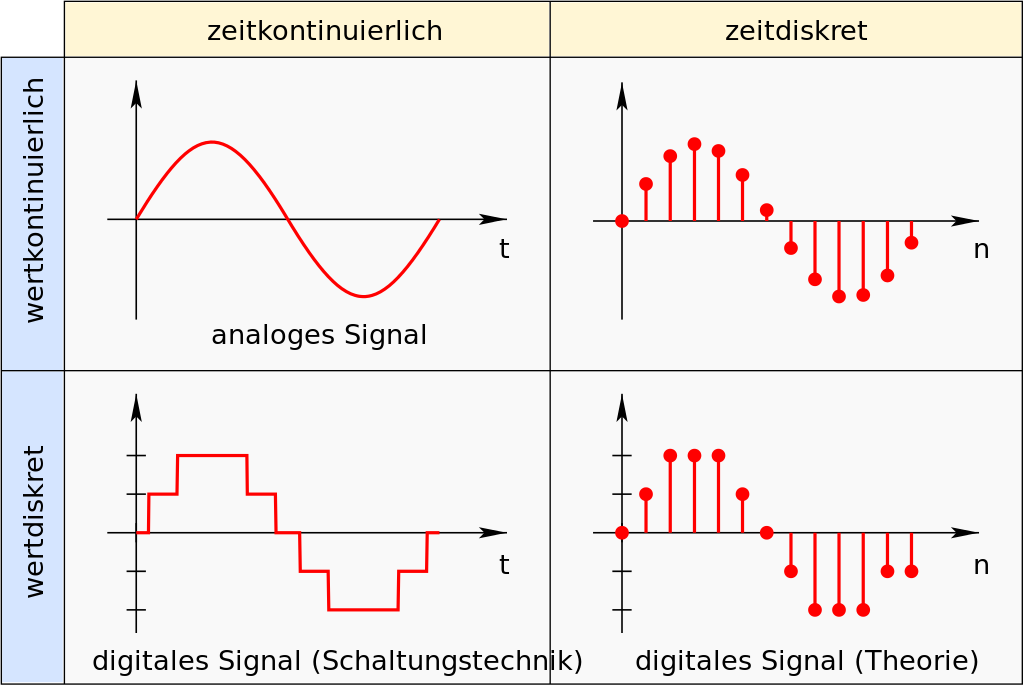
\includegraphics[scale=0.4]{images/signals.png}
\captionsource{Übersicht diskreter und kontinuierlicher Signale}{\cite[p. 2]{frey2008signal}}
\label{signals}
\end{figure}
Grundlegend existieren vier Formen, in denen ein Signal vorliegen kann. Dies wird in \ref{signals} dargestellt. Sowohl im zeit- als auch im Wertebereich können Datenpunkte in diskreter- sowie kontinuierlicher Form vorliegen. Geht man von einer rein kontinuierlicher Form der natürlich existierenden Werte aus, beispielsweise akustische Signale oder auch Temperatur, so besitzen all diese Signale eine zeit- als auch wertkontinuierliche Form.\\
Es existieren Ansätze in der Physik, nach welchen Zeit oder auch Distanz ein rein diskretes Konstrukt beschreiben, da diese eine beliebig kleine, jedoch konstante minimale Einheit besitzen. Auf diese Fragestellung wird hier jedoch nicht eingegangen, und somit wird angenommen, dass ein kontinuierlicher Zeitbereich existieren kann.\\
\newpage

\subsubsection{Ideale Abtastung}
\begin{definition}{Abtastrate}\\
Wird ein Signal im gleichmäßigem Abstand T erfasst, so beschreibt $\frac{1}{T}$ die Abtastfrequenz. Der n-te Wert liegt bei $t = n \cdot T$ vor.
\end{definition}

Bei der idealen Abtastung wird ein Dirac-Kamm, also eine Folge von Dirac-Stößen $\delta(t)$ genutzt. Liegt nun ein Signal $s(t)$ vor, so ergibt sich das abgetastete Signal wie folgt:\\
$s_a(t) = s(t) \cdot \sum\limits_{n=-\infty}^{\infty} \delta(t - nT)$\\
Dies ist jedoch lediglich ein mathematisches Konstrukt, und in der Anwendung kann dieses nicht genutzt werden. Im Folgenden wird die reale Abtastung behandelt.

\subsubsection{Reale Abtastung}
In der Realität existieren keine idealen Dirac-Stöße, da diese unendlich steile Flanken besitzen würden. Stattdessen 



Die Diskretisierung im Zeitbereich wird realisiert, indem eine Größe in beliebigen, jedoch äquidistanten Zeitintervallen $T$ erfasst wird. Das Inverse dieser Intervalle wird als 'Abtastrate' bezeichnet, also $\frac{1}{T}$.\\

\subsubsection{Quantisierung}
Im Wertebereich wird dieses Verfahren als 'Quantisierung' bezeichnet. Dies ist zunächst keine Form der Abtastung, ist jedoch eng mit dieser verwandt und wird somit kurz beschrieben.\\


Zunächst wird eine Auflösung $\delta$ gewählt, welche die Ordinate in äquidistante 'Stufen' einteilt. Jeder gemessene Wert wird zur Speicherung einer dieser Stufen zugeordnet, wobei in der Regel die Stufe mit dem geringsten Abstand zu dem Wert gewählt wird. Ein gemessener Wert $x$ wird mithilfe der im Folgenden beschriebenen Funktion einer Stufe zugeordnet.\\
$Q(x) = sgn(x) \cdot \delta \cdot \Big\lfloor \cfrac{|x|}{\delta} + \cfrac{1}{2} \Big\rfloor $\\
Hierbei beschreibt $sgn$ die Signum Funktion.\\
Für einen Wertebereich der Größe $l$ ergeben sich $N = \cfrac{l}{\delta}$ Stufen, welcher ein gemessener Wert zugeordnet werden kann. Es ist offensichtlich, dass mit einer genaueren (kleineren) Auflösung eine höhere Genauigkeit erzielt werden kann. Hierzu muss jedoch eine höhere Datenrate in Kauf genommen werten.



\subsection{Beweis}\label{3.2}
\subsection{Bedeutung}\label{3.3}

Nach der Abtastung eines Signals liegt dies zwangsweise in diskreter Form vor, sowohl im zeit- als auch im Wertebereich. Dies hat mehrere Ursachen. Zum einen existieren keine Messinstrumente, welche eine beliebige Größe beliebig genau messen können. So existieren beispielsweise High-End Sensoren, welche Temperaturen mit einer Auflösung von $\pm0.125^\circ C$ messen können und einer Genauigkeit von $\pm0.1^\circ C$ erfassen können. Es ist absehbar, dass diese Werte in Zukunft verbessert werden können, also Temperaturen genauer und mit einer geringeren Unsicherheit erfasst werden können. Jedoch zeigt sich auch, dass der praktischen Messung Grenzen gesetzt sind.\\
Die andere Problematik entspringt aus Speicherung gemessener Daten. Man nehme an, es existiere ein Messinstrument, welches beispielsweise Spannung beliebig genau messen könnte, und dies in beliebigen Zeitabständen. Wird nun eine Spannung gemessen und mit einer Genauigkeit von 15 Dezimalstellen gemessen, und dies geschieht mit einer Frequenz von $1M$Hz, so fallen $1 \cdot 10^6 \cdot 64$ bit $= 64 \cdot 10^6$ bit $= 8M$B an Informationen die Sekunde an. Dies wird auch als Datenrate bezeichnet.\\
Es ist offensichtlich, dass es somit nicht möglich ist, beliebig genau und häufig gemessene Daten zu speichern. Deshalb werden Daten diskretisiert.\\

\subsection{Periphere Schnittstellen}\label{3.4}
\subsection{Analoger und digitaler In-/Output}\label{3.5}